\documentclass[12pt,oneside,openany,letterpaper]{article}


\usepackage{fancyhdr}
\usepackage{helvet}
\usepackage{amsmath}
%\usepackage{graphicx}
\usepackage[pdftex]{graphicx}
\usepackage{psfrag}
\usepackage{setspace}
%\usepackage[hypertex, linktocpage]{hyperref}[2003/11/30]
\usepackage[linktocpage]{hyperref}[2003/11/30]
\usepackage{lscape}
\usepackage{nicefrac}
\usepackage{mathrsfs}
\usepackage{units}
\usepackage{upgreek}
\usepackage{amssymb}
\usepackage{color}
\usepackage{wrapfig}
\usepackage{multirow}
\usepackage{url}
\usepackage{verbatim}
\usepackage{textcomp}
\usepackage{epstopdf}
\usepackage{siunitx}

\onehalfspacing \setlength\textheight{667pt}
\setlength\textwidth{506pt} \setlength\oddsidemargin{-18pt}
\setlength\topmargin{-20pt}
%\setlength\footskip{24pt}
\addtolength\headheight{2.5pt} \addtolength\headsep{-14pt}
%\fancyhead[R]{\includegraphics[height=10.5pt]{ubclogo_bw.eps}\#:  55907968}
%\renewcommand\familydefault{\sfdefault}
\pagestyle{empty}

\newenvironment{packed_enum}{
\begin{enumerate}
  \setlength{\itemsep}{0pt}
  \setlength{\parskip}{0pt}
  \setlength{\parsep}{0pt}
}{\end{enumerate}}



\fancyhead[L]{\emph{Introduction to Electronics}}\fancyhead[R]{Diodes \& Rectifier Circuits}
\fancyfoot[L]{PHYS 231}\fancyfoot[R]{Experiment 6}
\pagestyle{fancy} \pagenumbering{arabic}

\begin{document}
\thispagestyle{plain}
\begin{center}
{\large{\bf{\fontfamily{phv}\selectfont Physics 231 - Diodes \& Rectifier Circuits (Exp.~6)}}}
\end{center}

\noindent In this lab you will build some simple rectifier circuits that can be used to convert AC signals which vary in time to constant DC voltages.

~

\noindent Diodes act as one-way valves for current: current can pass through the diode in one direction, but not the other.  In order for a diode to conduct, the potential at the p-type side must exceed the potential at the n-type side by at least $V_\mathrm{d}$, where $V_\mathrm{d}$ is typically between \SI{0.6}{} and \SI{0.7}{\volt} for silicon diodes.


~

{\bf 1. HALFWAVE RECTIFIER}

~

\noindent Construct the ``halfwave'' rectifier circuit shown in Fig.~\ref{fig:halfwave}.
\begin{figure}[h!]
\begin{center}
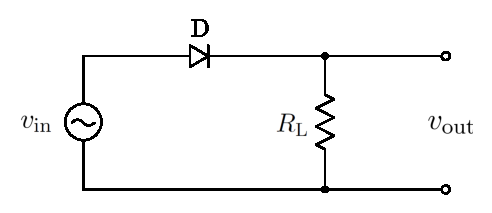
\includegraphics[width=.45\textwidth]{halfWave.eps}
\caption{\label{fig:halfwave}The halfwave rectifier.}
\end{center}
\end{figure}

\noindent (i) Use an IN4148 diode and $R_\mathrm{L}=\SI{1}{\kilo\ohm}$. Set your function generator to output a \SI{1}{\kilo\hertz} sine wave with an amplitude of \SI{10}{\volt} and observe $v_\mathrm{in}$ and $v_\mathrm{out}$ on the oscilloscope.  What is the peak value of $v_\mathrm{out}$?  Does this agree with what you'd expect?

~

\noindent (ii) Now also use a DMM to measure $v_\mathrm{out}$ (in parallel with the oscilloscope measurement).  Set the DMM to DC mode, which will measure the average value of $v_\mathrm{out}$.  Recall that the average value of a function over time interval $T$ is given by:
$$
\overline{f}=\frac{1}{T}\int_{t_0}^{t_0+T}f(t)\,dt.
$$  
Use this expression to estimate the expected value of $\overline{v_\mathrm{out}}$ over one period.  Does your calculation agree, within reason, with the measured DC voltage.

~

\noindent (iii) Now set the DMM to AC voltage mode to measure the rms value of $v_\mathrm{out}$.  Record the value.

\clearpage

{\bf 2. IMPROVED HALFWAVE RECTIFIER}

~

\noindent Add a \SI{1}{\micro\farad} capacitor in parallel with $R_\mathrm{L}$ as in Fig.~\ref{fig:halfwaveC}.
\begin{figure}[h!]
\begin{center}
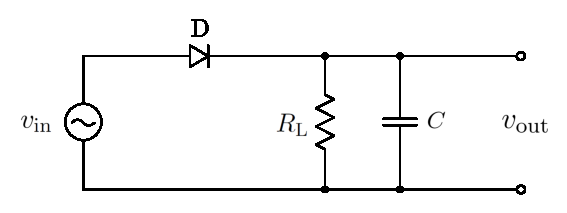
\includegraphics[width=.53\textwidth]{halfWaveC.eps}
\caption{\label{fig:halfwaveC}The halfwave rectifier with parallel capacitor at the output.}
\end{center}
\end{figure}

\noindent (i) Measure the peak voltage of $v_\mathrm{out}$.  How does it compare to 1(i)?

~

\noindent (ii) Measure the DC voltage of $v_\mathrm{out}$.  How does it compare to 1(ii)?

~

\noindent (iii) Measure the rms voltage of $v_\mathrm{out}$.  How does it compare to 1(iii)?

~

\noindent (iv) Let's call the DC component of $V_\mathrm{DC}$ and the AC component $v_\mathrm{rms}$.  We can then define a quantity called the ``ripple factor'' as $r=v_\mathrm{rms}/V_\mathrm{DC}$.  In a high-quality rectified circuit (or AC-to-DC converter) one desires $v_\mathrm{rms}\ll V_\mathrm{DC}$ such that $r$ is very small.

~

\noindent Measure $r$ for the circuit in Fig.~\ref{fig:halfwaveC} for 10 frequencies between \SI{1}{\kilo\hertz} and \SI{10}{\kilo\hertz}.  Make a plot of $r$ versus $1/f$.  You will show that $r$ and $f$ are inversely related in one of your assignments.

\clearpage

{\bf 3. FULLWAVE RECTIFIER}

~

\noindent Construct the ``fullwave'' rectifier circuit shown in Fig.~\ref{fig:fullwave}.
\begin{figure}[h!]
\begin{center}
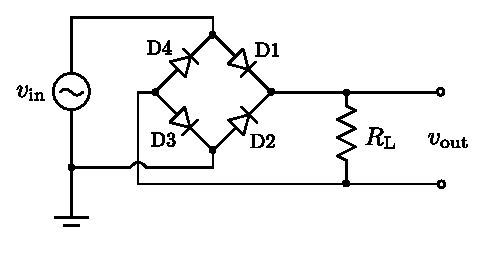
\includegraphics[width=.51\textwidth]{fullWave.eps}
\caption{\label{fig:fullwave}The fullwave rectifier.}
\end{center}
\end{figure}

\noindent (i) Again, use an IN4148 diodes and $R_\mathrm{L}=\SI{1}{\kilo\ohm}$. Set your function generator to output a \SI{1}{\kilo\hertz} sine wave with an amplitude of \SI{10}{\volt}.  In order to observe $v_\mathrm{out}$ on the oscilloscope, you will have to use both channels and math mode.  You will note be able to simultaneously observed $v_\mathrm{in}$ on the oscilloscope.  You should now see clearly why the first circuits in parts 1 and 2 are known as the halfwave rectifiers and the circuit in Fig.~\ref{fig:fullwave} is known as a full wave rectifier. 

\clearpage

{\bf 4. IMPROVED FULLWAVE RECTIFIER}

~

\noindent  Add a \SI{1}{\micro\farad} capacitor in parallel with $R_\mathrm{L}$ as in Fig.~\ref{fig:fullwaveC}.
\begin{figure}[h!]
\begin{center}
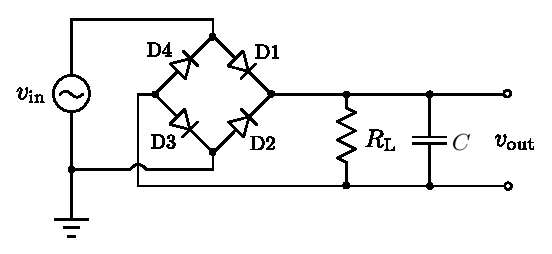
\includegraphics[width=.6\textwidth]{fullWaveC.eps}
\caption{\label{fig:fullwaveC}The fullwave rectifier with parallel capacitor at the output.}
\end{center}
\end{figure}

\noindent (i) Measure the peak voltage of $v_\mathrm{out}$. How does it compare to 2(i)?

~

\noindent (ii) Measure the DC voltage of $v_\mathrm{out}$. How does it compare to 2(ii)?

~

\noindent (iii) Measure the rms voltage of $v_\mathrm{out}$. How does it compare to 2(iii)?

~

\noindent (iv) What path does the current take when $v_\mathrm{in}$ is positive and greater than $V_\mathrm{d}$?  Which diodes are conducting and which ones are not conducting?

~

\noindent (v) What path does the current take when $v_\mathrm{in}$ is negative and its magnitude is greater than $V_\mathrm{d}$?  Which diodes are conducting and which ones are not conducting?
 

\end{document}
